\begin{figure}[!ht]
\centering
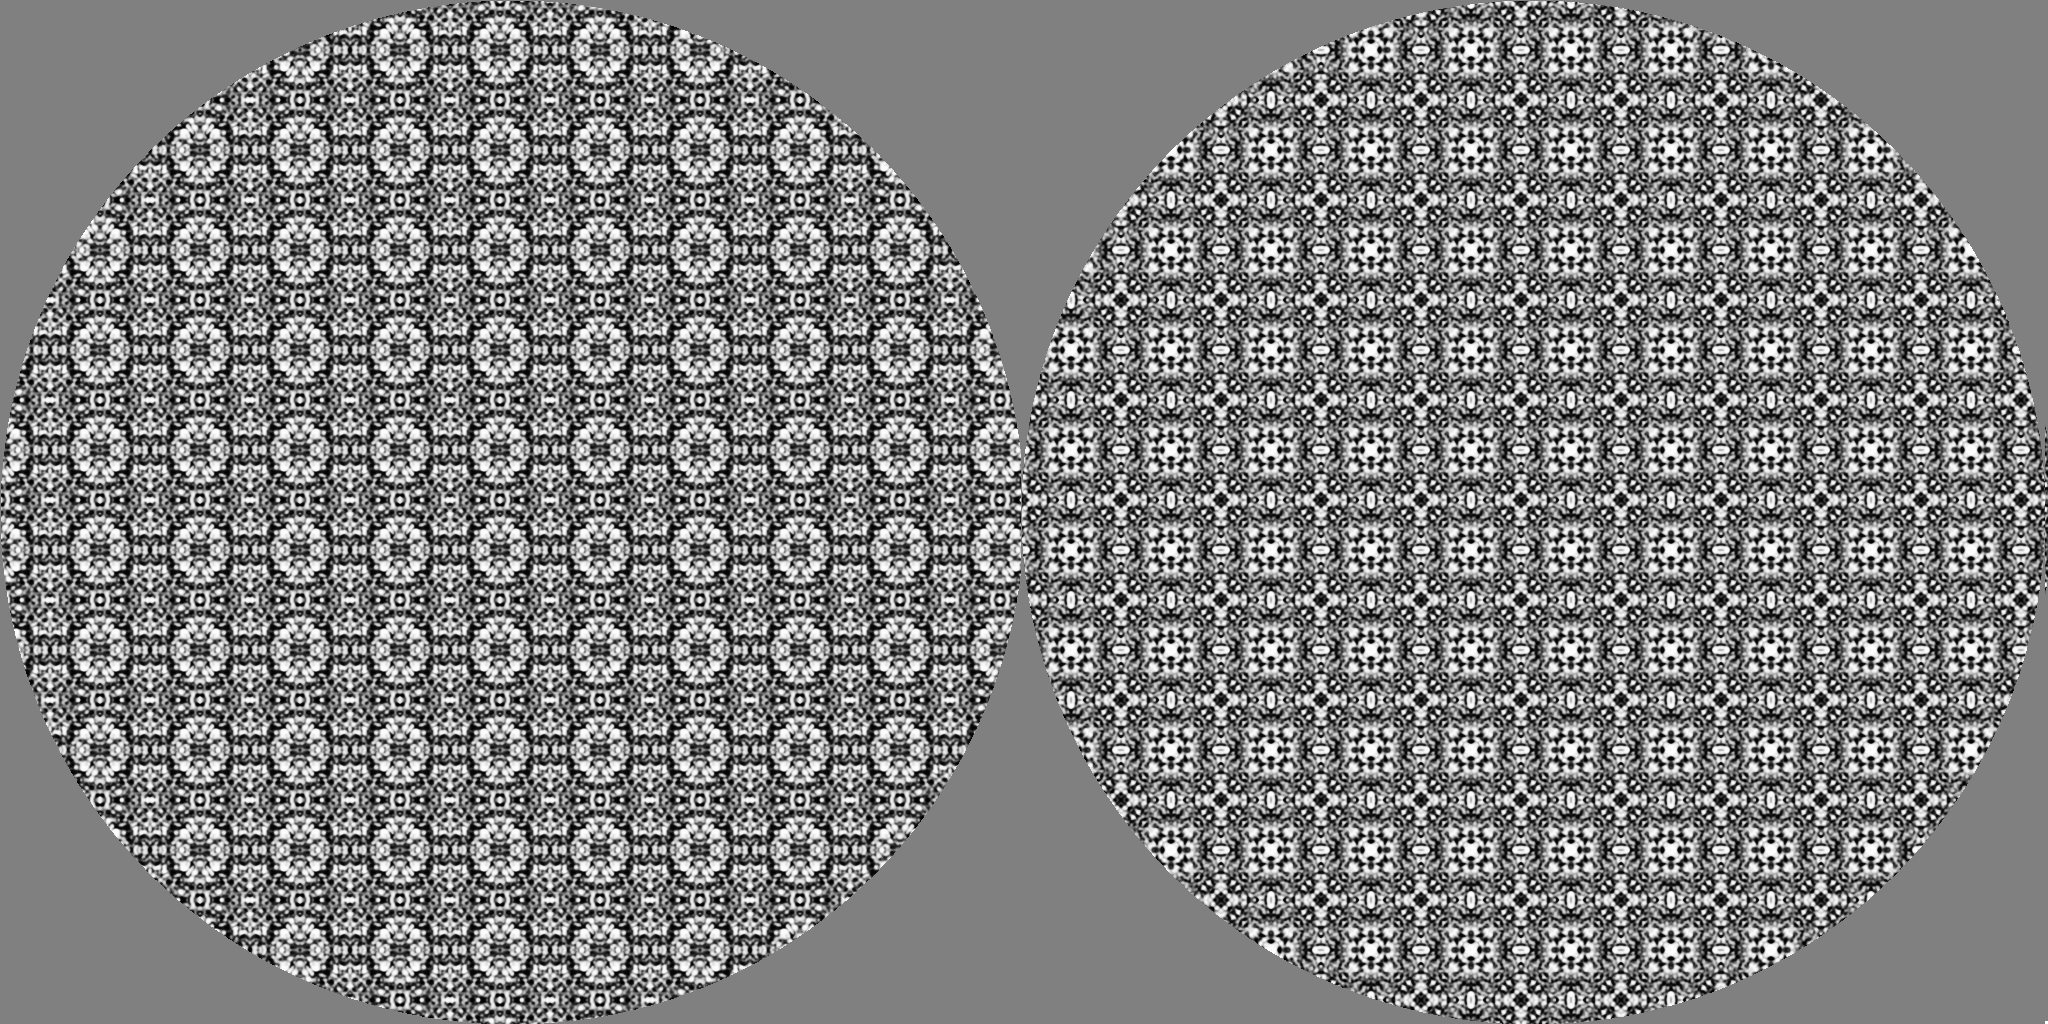
\includegraphics[width=0.9\columnwidth]{pmmp4m}
\caption{PMM on the left (note the tiles lack reflection on the horizontal axis, but have it on the vertical axis), P4M on the right.}
\label{pmmp4m}
\end{figure}

\begin{figure}[!ht]
\centering
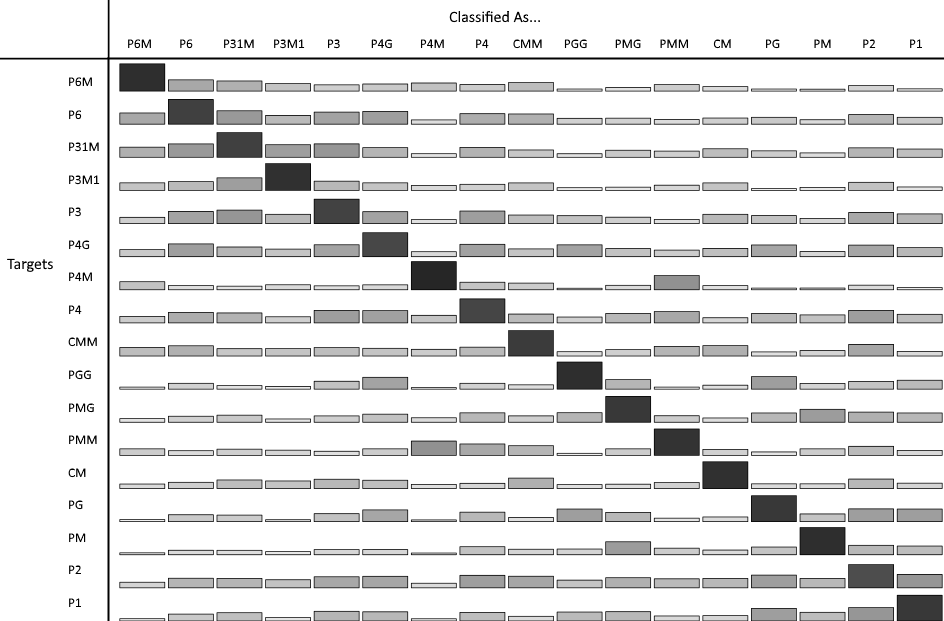
\includegraphics[width=0.9\columnwidth]{accuracies-grayscale}
\caption{On the vertical we have the targets. On the top are the distracters. The bars represent the percentage of errors. The main diagonal, where the target and distracter are the same, represents the aggregate accuracy in labeling that group correctly. The darkness of the bar also corresponds to its value (higher is darker).}
\label{fullacc}
\end{figure}